\documentclass{article}
\usepackage[german]{babel}
\usepackage[utf8]{inputenc}
\usepackage{tabularx}
\usepackage{listings}
\usepackage{graphicx}
\usepackage{float}
\usepackage{url}

\usepackage[
  style=alphabetic, % Loads the bibliography and the citation style
  % bibstyle=alphabetic, % load a bibliography style
  % citestyle=alphabetic, % load a citatio style
  natbib=true, % define natbib compatible cite commands
%%--- Backend --- --- ---
  backend=biber,   % (bibtex, biber)
  bibwarn=true,     %
  texencoding=auto, % auto-detect the input encoding
  bibencoding=auto, % (auto (equal to tex), <encoding>)
]{biblatex}
\addbibresource{references.bib}

\title{Projektbericht TranscriptionDesk}
\author{Robert Rößling, Jakob Runge, Oliver Schurig, Franz Teichmann}
%\date{März 2015}

\begin{document}
%TODO: Stets zwei-drei Sätze Kapiteleinleitung beachten, englische Fachbegriffe auf ein Minimum reduzieren und nicht mehrere Begriffe für eine Semantik nutzen
% z.B. Nutzer statt User, Projekt statt Praktikum
%TODO genaue Beschreibung des Projektes erfolgt erst nach der analyse und Einordnung

\maketitle

\subsection*{Abstract}
Das TranscriptionDesk Projekt umfasste Konzeption und Entwicklung einer webbasierten Plattform,
auf der sich unterschiedlich versierte Nutzer zwecks Mitarbeit an der Transkription
einer großen Datenbasis aus Scans mittelalterlicher Handschriften registrieren können.
Dies umfasst außerdem die Analyse der Scans in Bezug auf die Unterscheidung zwischen Originaltext und nachträglicher Annotation.
Alle Quelldateien mit Dokumentation, Installationsanleitung und diesem Projektbericht
stehen unter MIT Lizenz und sind digital veröffentlicht unter \url{https://github.com/runjak/TranscriptionDesk}.

\tableofcontents
\newpage

%omeka-login: für jeden Scan ist die Herkunft mit drin
%CCBI NDNC für die meisten
\section{Einleitung}
Das Projekt TranscriptionDesk wurde im Zuge des Moduls ,,Citizen Science'' an der Universität Leipzig im Sommerstemester 2015 durchgeführt.
Das Thema umfasste die Konzeption und Entwicklung einer Plattform nach dem Paradigma der Citizen Science,
die eine dynamische Transkription einer großen Datenbasis aus Scans mittelalterlicher Handschriften durch zahlreiche Nutzer ermöglicht.

In dieser Arbeit sollen die Hintergründe sowie unsere Ideen und Gedankengänge auf dem Weg vom Thema zum konkreten Projektauftrag,
die von uns betrachteten (Teil-)Aufgaben sowie die Ergebnisse präsentiert
und eine Übersicht über die Architektur der entstandenen Software gegeben werden.
Dazu sollen zunächst die theoretischen Grundlagen erläutert werden,
um daraus im Anschluss unsere Projektdefinition abzuleiten und die Überlegungen aus der Planungsphase zusammenzufassen.
Danach soll ein direkter Einstieg ins Projekt mit der Darstellung der Architektur und der Produktfunktionen erfolgen und auf Funktionen hingewiesen werden,
welche bisher aufgrund des begrenzten Zeitrahmens weniger berücksichtigt werden konnten.
Am Schluss des Berichtes wird eine Zusammenfassung der ,,lessons learned'' sowie ein Ausblick auf mögliche Folgeprojekte gegeben.

\section{Theoretische Grundlagen}
In diesem Kapitel sollen die Grundlagen für die späteren Erläuterungen gelegt werden.
Dazu soll zunächst die Definition von Citizen Science aus der Vorlesung rekapituliert und auf verschiedene Deutungen des Begriffes eingegangen werden,
um anschließend eine Arbeitsdefinition als Plan für unser Projekt abzuleiten und diesen in die Kategorien der Citizen Science nach Crowston und Wiggins einzuordnen.
Dazu sei auch auf Literatur zum Thema verwiesen.

Es handelt sich bei ,,Citizen Science'' um einen verhältnismäßig neumodischen Begriff
für ein gleichnamiges Teilgebiet der angewandten Sozialwissenschaften und Geisteswissenschaften,
welches nur schwerlich genau abzugrenzen ist. Anwendungsmöglichkeiten und die Komplexität dieses Themengebietes
wurden uns im Laufe der Lehrveranstaltung an aktuellen sowie an historischen Beispielen veranschaulicht
und sowohl Gemeinsamkeiten als auch Unterschiede zwischen den verschiedenen in den Beispielen verfolgten Ansätzen herausgearbeitet.
Da es keine ,,einfache'' oder ,,schnelle'' Definition gibt, die diesen Sachverhalt vollständig beschreibt,
versuchen wir die Komplexität noch einmal in den zwei folgenden Unterkapiteln einzufangen
und einer Definition so nahe zu kommen, wie es uns möglich ist.

\subsection{Definition Citizen Science}
Die Frage, wie sich Citizen Science definieren lässt, ist also keine, die sich leicht beantworten lässt.
Festgehalten wurde bereits, dass der Begriff erst seit jüngerer Zeit verwendet wird.
Das bedeutet jedoch nicht im gleichen Zuge, dass die Idee der Citizen Science eine neue Erfindung ist.
Tatsächlich lassen sich Aktivitäten, die heutzutage unter diesem Begriff zusammengefasst werden,
mit dem heutigen Wissensstand fast 200 Jahre in die Vergangenheit zurückverfolgen. Die präzisere Frage lautet also womöglich:
,,Wer oder was genau ist eigentlich ein Citizen Scientist?''

Das versucht beispielsweise Wiederhold\cite{Wiederhold} (S.703-4) zu beantworten.
Zum einen werden dazu aktuelle Entwicklungen, wie etwa das relativ bekannte FoldIt-Spiel \footnote{FoldIt ist ein Onlinespiel,
das sich mit Proteinfaltung befasst. Der Spieler benötigt keinerlei biologisches Hintergrundwissen.
Spielergebnisse liefern wertvolle Daten für Wissenschaftler und haben bereits zu Erkenntnissen in der Virenforschung geführt.
\url{https://fold.it/portal/}}, sowie historische Gegebenheiten erwähnt, die in die Citizen Science eingeordnet werden.
Eines der ältesten bekannten Projekte, so Wiederhold, ist das National Audubon Society's Christmas Bird Count-Projekt,
dessen Spuren sich bis in die heutige Zeit ziehen, wie die dazu existierende Homepage\footnote{Das Projekt wurde 1900 von Frank M. Chapman gegründet.
Ziel war es, Vogelarten zu bestimmen und zu zählen, um der bis dahin üblichen ,,Side Hunt'',
die jedes Jahr zur Weihnachtszeit Jäger dazu herausforderte, so viele Vögel wie möglich zu schießen,
eine umweltverträgliche Alternative zu bieten. \url{https://www.audubon.org/conservation/science/christmas-bird-count}} uns zeigt.

Diese zwei Beispiele zeigen gleichzeitig auch eine Verlagerung der Citizen Science aus der Umwelt in die digitale Welt.
Obwohl viele bekannte Projekte weiterhin unter der ,,Environmental Science'', wie Wiederhold sie nennt, einzuordnen sind,
besteht in einer großen Anzahl der Projekte die Arbeit für den Citicen Scientist nur aus nicht maschinell abstrahierbarer Computerarbeit,
welche wenig bis keine Vorkenntnisse erfordert.

Unter Berücksichtigung der bis hierhin erwähnten Fakten, könnte man also bereits versuchen, den Citizen Scientist zu definieren.
Dies tut Wiederhold schon im ersten Satz ihres Artikels,
in dem sie Cohn zitiert: ,,The term 'citizen scientists' refers to volunteers who participate as field assistants in scientific studies.
Citizen scientists...are not paid for their assistance, nor are they necessarily even scientists.'' \cite{Cohn} (58:192-7).
Dabei scheint diese Definition auf den ersten Blick überraschend treffend die Umstände zu beschreiben,
unter denen ein solcher Citizen Scientist arbeitet und in welche Themengebiete er sich einbringt.
Zugleich wird jedoch auch ein Aspekt ausgespart, der für uns an dieser Stelle wesentlich erscheint:
Allein durch den Versuch einer Definition eines Citizen Scientists, ist das Gebiet der Citizen Science noch längst nicht umgrenzt.
Fragen die nicht beantwortet werden, sind beispielsweise solche nach dem Rahmen bei der Bestimmung einer Forschungsfrage,
eines Projektzieles, oder auch welche Finanzierungsmöglichkeiten für solche Projekte bestehen.
Wie genau ist es mit der Wissenschaftlichkeit des Projektes zu nehmen und muss es einem gesellschaftlichen, also eher wohltätigen,
Zweck dienen oder darf es auch einen wirtschaftlichen Charakter aufweisen?
Wo ist die Grenze zum Crowdsourcing\footnote{Crowdsourcing: Bezeichnend für das Auslagern interner Aufgaben eines Unternehmens an Freiwillige Nicht-Angestellte.
Angelehnt an den Begriff Outsourcing, bei dem Drittunternehmen ausgelagerte Aufgaben verrichten. Häufig wird Crowdsourcing über das Internet reaöosoert.} zu ziehen?

Um diese Fragen für uns beantworten zu können, befassten wir uns mit unterschiedlichen, bereits existierenden Projekten.
Einige davon gehörten eindeutig zum Crowdsourcing, andere wiederum waren für uns nicht so eindeutig einzuordnen und haben die Meinungen durchaus geteilt.
Gewissermaßen kann man also Crowdsourcing und Citizen Science als zwei gegensätzliche Pole betrachten, die allerdings einen fließenden Übergang besitzen.
Dieser Meinung ist auch Haklay\cite{Haklay} (pp 105-122), der diese Grauzonen in unterschiedliche Ebenen einteilt.
Darauf werden wir im folgenden Kapitel näher eingehen.
Somit wäre Citizen Science also nur die eine Seite der Medaille
- eine Form der Beteiligung durch nicht spezifisch qualifizierte Menschen aus der breiten Bevölkerung im Rahmen ihrer Freizeit,
die sich eher vom Crowdsourcing zu distanzieren versucht.
\newline
Auch Crowston und Wiggins\cite{CW} versuchen sich an einer eigenen Definition von Citizen Science.
Im Rahmen ihrer Untersuchung hielten sie fest, dass sich das Spektrum der Projekte in fünf Kategorien unterteilen lässt:
,,Based on the clustering, we identified five mutually exclusive and exhaustive types of projects,
which we labelled Action, Conservation, Investigation, Virtual and Education'' (S. 5).
Auch diese sollen im Folgekapitel noch einmal einzeln Erwähnung finden.
Unter Berücksichtigung dieser Kategorisierung fällt es womöglich schon um einiges leichter,
sich ein Bild vom Charakter der Citizen Science zu machen.
Ein letzter Definitionsversuch, der hier Erwähnung finden soll, kommt ebenfalls von Cohn,
als ,,die wissenschaftlichen Aktivitäten in denen nicht-professionelle Wissenschaftler sich freiwillig an Datensammlung,
Analyse und Verbreitung eines wissenschaftlichen Projekts.''\cite{Cohn}.%dieser Satz kein Verb? FIXME
An dieser Definition lassen sich vor allem zwei bemerkenswerte Tatsachen finden. Zum einen ist es ein Versuch,
sich über die Definition eines Citizen Scientists zu definieren. Zum anderen wird ausdrücklich darauf aufgebaut,
dass es sich bei Citizen Science um eine wissenschaftliche Tätigkeit handelt.
Ob dies einer Tatsache in Sachen Definition entsprechen muss ist unserer Auffassung nach eine Auffassungssache,
da es auch Projekte gibt, deren Wissenschaftlichkeit angezweifelt werden kann,
deren Einordnung in die Kategorie der Citizen Science für uns durchaus ein Diskussionsthema war.
Ein Beispiel könnte das ReClam The Bay Projekt\footnote{ReClam The Bay: Projekt zur Stärkung der Muschelpopulation an bestimmten Stränden.
\url{www.reclamthebay.org}} sein, das durchaus ein sinnvolles Ziel verfolgt und Aufklärung betreibt,%sinnvoll subjektiv? FIXME
das jedoch an erster Stelle ein umweltveränderndes Ziel verfolgt und keine wissenschaftlichen Daten erhebt oder anderen wissenschaftlichen Nutzen aufbaut.
\newline
Bevor wir versuchen, unser Projektthema im Rahmen der Citizen Science einzuordnen,
möchten wir noch einige Ansichten bezüglich der Einteilung der Citizen Science in unterschiedliche Kategorien beleuchten.

\subsection{Kategorien der Citizen Science}
Wie bereits erwähnt, machte sich auch Haklay Gedanken über die Möglichkeiten, Citizen Science vom Crowdsourcing zu trennen.
Seine Überlegungen nach existiert eine Skala, welche das Crowdsourcing nur als das eine Extremum betrachtet und diesem die ,,Extreme Citizen Science'' entgegenstellt.
Die intesanntesten Ebenen liegen im Spektrum zwischen diesen beiden. Die vier Kategorien untergliedern sich wie folgt:

\begin{description}
\item[Level 1: Crowdsourcing.]
Hier beruht die Computerarbeit auf freiwilliger Basis.
Die einfache Bürgerschaft dient lediglich als Sensor, andere Aufgaben werden von anderer Seite aus erledigt.
\item[Level 2: Distributed Intelligence.]
Auf diesem Level sollen Freiwillige Denkarbeit verrichten und werden dabei grundlegend für Interpretative Aufgaben eingesetzt.
\item[Level 3: Participatory Science.]
In dieser Kategorie werden die Freiwilligen bereits in der Problemdefinition mit einbezogen, sie übernehmen aber auch Aufgaben zur Sammlung von Daten.
\item[Level 4: Extreme Citizen Science.]
Diese Kategorie betrachtet den gesamten wissenschaftlichen Prozess als kollaborative Aufgabe für die freiwillige Teilnehmerschaft.
Sie nimmt an der Problemdefinition ebenso teil wie an der Sammlung von Daten und deren Analyse.\cite{Haklay} (pp 115)
\end{description}

Während Haklay versucht, den Unterschied der Citizen Science nach außen abzugrenzen, gibt es auf der anderen Seite auch Überlegungen,
wie die Citizen Science sich nach Innen hin aufteilen lässt. Wie bereits im vorangehenden Unterkapitel erwähnt wurde,
fanden Crowston und Wiggins fünf Cluster unterschiedlicher, bereits existierender Projekte, die zumindest von sich behaupten,
in die Kategorien der Citizen Science zu gehören.

\begin{description}
\item[Action:]
Bei Action handelt es sich um Projekte, die ihren Ursprung häufig in einem lokal angesiedelten Beweggrund sehen.
Sie werden nicht durch Wissenschaftler in die Wege geleitet,
sondern viel eher durch einfache Leute, die einen Handlungsbedarf sehen und eine Bewegung für Freiwillige ins Leben rufen.
Für gewöhnlich geht es dabei um Ziele, welche die Umwelt betreffen.
Technologien kommen dabei nur minimal zum Einsatz, soweit sie von Notwendigkeit sind.
\item[Conservation:]
Conservation befasst sich mit dem Management der natürlichen Ressourcen.
Freiwillige haben dabei häufig Verwaltungsaufgaben oder sind dafür zuständig, eine breitere Masse zu erreichen.
Folglich ist auch Wissensvermittlung ein explizites Ziel, welches mit dieser Projektgruppierung einhergeht.
Finanzierung ist oft ein Problem, das nur über staatliche Gelder gelöst werden kann und somit eine starke Abhängigkeit aufbaut.
\item[Investigation:]
Investigation hat wissenschaftliche Untersuchungergibnisse zum Ziel.
Hier werden Daten von Freiwilligen im physikalischen Umfeld gesammelt.
Bildung ist hier zwar kein Ziel, oft jedoch ein Faktor, der die Arbeit erheblich genauer (und somit besser auswertbar) und effizienter gestaltet.
Gleichzeitig ist Bildung auch ein durchaus gewöhnlicher Nebeneffekt der Arbeit mit der Materie.
\item[Virtual:]
Virtual weist viele Parallelen zu Investigation auf, spielt sich jedoch statt in einer physikalischen, in einer virtuellen Umgebung ab.
Gerade hier ist es nicht so leicht, die Teilnehmer als Citizen Scientists wahrzunehmen, da sie oft nur eine Instanz sind, die Daten verarbeitet und validiert.
Probleme, mit denen man sich hier befassen muss ist die Validierung der Daten, da es auch unausweichlich eine Fehlerrate gibt,
und die große Masse an Nutzern, die auf den komplexen Plattformen agiert, zu behandeln.
\item[Education:]
Education hat, wie der Name vermuten lässt, einen primären Bildungsauftrag zum Ziel.
Nicht immer ist es dabei leicht, Gelder zu erhalten, welche die hohen Kosten decken.
Vor allem aus dem Grund, dass kaum Daten generiert werden, die in irgendeiner Form nutzbar wären, wird kein wirtschaftlicher Mehrwert generiert,
was die Finanzierung umso mehr erschwert.
\end{description}
Sicher lassen sich noch wesentlich mehr Kategorien für konkrete Anwendungs-fälle finden,
doch für den Zweck der Charakterisierung und Einordnung unseres Projektes sollen die Arbeiten von Haklay sowie Crowston und Wiggins als repräsentative Beispiele genügen.

\subsection{Einordnung unseres Projektes}
Unserer Einschätzung nach ist TranscriptionDesk aufgrund der Aufgabenstellung durchaus als Citizen Science und nicht als Crowdsourcing zu betrachten.
Betrachten wir unseren Standpunkt durch Haklays Augen, so würden wir unser Projekt auf Level 2, der ,,Distributed Intelligence'' einordnen,
da Freiwillige ganz zur Interpretation der Texte eingesetzt werden sollen und somit ihre Denkleistung in Anspruch genommen wird.
Außerdem ist die Problemdefinition bereits vorgegeben, so dass wir das Projekt auch nicht auf Level 3 einordnen könnten.
Man sollte dennoch Notiz davon nehmen, dass wir damit dem Crowdsourcing nach Haklay sehr nahe kommen.%damit genauer ausführen FIXME

Schauen wir uns die Kategorien von Crowston und Wiggins an, so müssen wir TranscriptionDesk zwangsläufig zur Kategorie ,,Virtual'' zählen.
Alle Faktoren des Projektes treffen genau zu.
Lediglich einige wenige Faktoren der Action-Kategorie werden ebenfalls erfüllt, da Beispielsweise der Ursprung des Projektes darin liegt,
dass Daten vorhanden sind, die transkribiert und validiert werden müssen und somit der Beweggrund für das Projekt darin lag,
dass die Notwendingkeit zum Handeln erkannt wurde.
Der wesentlichste Unterschied ist nur, dass es keinen lokalen, umweltbezogenen Handlungsfaktor gab, der Ausschlag dafür gegeben hat.
Somit ist ,,Virtual'' die einzig zutreffende Kategorie.

\section{Projektübersicht}
In diesem Kapitel soll mit einer detaillierten Übersicht über das Projekt und dessen Zielstellung ein direkter Einstieg geben werden.
Dazu soll ausgehend von der Projektvision die Struktur der Datenbasis erläutert und die erwartete Nutzerbasis reflektiert werden.

\subsection{Ziele}
Unser Projektthema fand seine Motivation in der Abteilung der Digitalen Geistes-wissenschaften der Universität Leipzig.
Dort liegen tausende Scans mittelalter-licher Schriftstücke vor, deren Informationsgehalt ohne vorherige Transkription nicht digital zu verarbeiten ist.
Es wurde als unmöglich bewertet, den Inhalt der Schriftstücke mittels typischer Optical-Character-Recognition-Methoden (OCR) sinnvoll zu digitalisieren.
Das hat im Wesentlichen zwei Gründe.

Einerseits war Papier im Mittelalter eine Mangelware und somit ein wertvolles Gut, das sparsam verwendet wurde.
Deswegen nutzte man freien Platz gut aus und es gibt Passagen,
die nicht in einen gemeinsamen zeitlichen Kontext gehören (z.B. nachträgliche Annotationen) und somit händisch getrennt werden müssen.
Der Fakt, dass die Schriftstücke aufgrund ihres Alters bereits durch viele Hände gegangen sind und im Laufe der Zeit
mit unterschiedlichen Handschriften auf dem Papier gearbeitet wurde, erschwert dies umso mehr.
Diese Informationen sollen entsprechend getrennt und digitalisiert werden.

Der zweite Grund besteht darin, dass das Schriftbild des Mittelalters oft künst-lerisch aufgewertet wurde.
So waren Texte in Blockform sehr beliebt und man erfand allerlei unterschiedliche Formen für semantisch gleichbedeutende Buchstaben,
die durch ihre Vielfalt für einen OCR-Algorithmus praktisch unmöglich zu lesen sind.

Die Aufgabe, welche sich daraus ergibt, kann praktisch nur durch akribische, händische Arbeit gelöst werden.
An dieser Stelle soll die Citizen Science ins Spiel kommen:
Durch den Aufbau einer Webplattform könnte ein großer Teil der kleinlichen Arbeit nach außen,
an Freiwillige mit unterschiedlichen Erfahrungen und unterschiedlichem Wissen abgegeben werden.
Dadurch soll die Digitalisierung der auf den Scans enthaltenen Texte nicht nur beschleunigt, sondern womögliche sogar erst ermöglicht werden.

Das Ziel, das wir vor Augen haben ist also der Aufbau einer Weboberfläche, welche die Scans an eine offene Gruppe freiwilliger Nutzer bereitstellt,
ihnen die Werkzeuge für deren Bearbeitung bereitstellt, die Ergebnisse speichert, und der Nutzerschaft die Möglichkeit bietet,
ihre gegenseitigen Ergebnisse zu bewerten, um ein einheitliches Level an Validierung der digialisierten Texte anzustreben.
Die Seite soll so strukturiert sein, dass sie weitestgehend selbstverwaltend ist und lediglich einige wenige Administratoren
die wenigen verbleibenden Verwaltungsaufgaben erledigen können.
Dabei ist auch die Möglichkeit gegeben, diese Administratoren ebenfalls in Teilen aus der Nutzerbasis zu beziehen.

Die Arbeit für einen Nutzer soll aus zwei unterschiedlichen Aufgaben bestehen.
Erstere besteht darin, Rechtecke auf den Scans zu ziehen, um ,,Areas of Interest'' zu markieren.
Diese können beispielsweise Bilder oder zusammengehörende Textfetzen sein.
Das Ergebnis ist eine Interest Map eines Scans, die andere Nutzer bewerten können, um deren Akzeptanz wiederzuspiegeln.
Scans können direkt ausgewählt oder per Zufall zugeordnet werden.

Die zweite Aufgabe besteht dann aus der eigentlichen Transkription.
Eine Interest Map wird verwendet und die darauf enthaltenen Areas of Interest werden vom Nutzer mit einer Transkription versehen.
Auch dieses Ergebnis lässt sich speichern und bewerten und somit wird ein bestes Ergebnis ermittelbar.
Unsere Aufgabe ist es dabei, all diese Funktionen als Grundfunktionalität zu implementieren und sie ansprechend zu gestalten.
Der letzte Punkt ist für uns sehr wesentlich, da uns bekannt ist, dass ähnliche (und darunter technisch gesehen sehr gute)
Projekte bereits an kleinen Schönheitsfehlern scheitern mussten, weil die Nutzer sich einfach nicht angesprochen fühlten.
Zusätzlich gehört es aus mehreren Gründen zu unserem Ziel, eine Login-Routine für das User-Management aufzubauen.
Dies bietet viele Vorteile beim Verfolgen von Veränderungen, für eine faire Verteilung von Bewertungen,
oder etwa um Statistiken einzelner oder auch aller Nutzer zu erstellen.
Außerdem besteht eine unserer wichtigsten Aufgaben darin, auf der gesamten Weboberfläche Unicode verwendbar und lesbar zu machen.
Ganz speziell bedeutet das, das wir eine sehr umfangreiche Eingabemaske aufbauen müssen,
die einen mächtigen Satz an mittelalterlichen Sonderzeichen in einer nutzerfreundlichen Art und Weise hergibt.
Die Identifikation von Scans erfolgt über Cite URNs.% Quelle für Cite URNs zitieren! FIXME
Wir wollen die Areas of Interest durch Erweiterung des Konzeptes ebenfalls über jene Cite URN identifizieren können.
%<Irgendwas wichtiges vergessen? Hier ist die richtige Stelle>

Die bisher genannten Features haben die höchste Priorität und bilden die Grundfunktionalität unserer Weboberfläche.
Ab diesem Punkt lassen sich schrittweise weitere Features hinzufügen um die Arbeit zu erleichtern, angenehmer oder einfach ansprechender zu gestalten.
Deswegen haben wir unsere anfängliche Planung mittels Scrum an ein agiles Entwicklungsmodell angelehnt.
Zuerst planten wir unsere grobe Architektur sowie diverse Technologien, die wir Verwenden könnten.
Auf beides werden wir in Folgekapiteln noch einen genaueren Blick werfen. Dann wurden drei Meilensteine geplant,
wobei der erste davon für die Erstellung der Nutzerauthentifikationsroutine und die Anbindung der im Hintergrund genutzten Diensten angedacht war.
Im zweiten Meilenstein ging es im Prinzip um alles, was die Maske der Weboberfläche sowie die Implementation der Arbeitswerkzeuge für die Nutzer betrifft.
Damit sollte die Grundfunktionalität weitestgehend aufgebaut sein. Für alle Eventualitäten soll es noch einen dritten Meilenstein geben,
in dem konkrete Bugs gelöst werden sollen und, falls dann noch ausreichend Zeit bleibt, direkt weitere Funktionen implementiert werden können.

%Warum haben wir <herp> gemacht?
%Rückbezug zu unserer Definition von Citizen Science.

\subsection{Struktur der Datenbasis}
Wie sehen unsere Dokumente und Rohdaten aus?
Wo kommen diese Daten her?
%Open Philology-Project letzten Jahres. Bei Omeka einloggen um Infos detailiert zu sehen. Falls dort nicht zu sehen, SOFORT THOMAS BESCHEIDGEBEN!

\subsection{Produkteinsatz / Erwartete Userbasis}
Ausgehend von der Motivation des Projektes sehen wir den vielversprechendsten Weg der Umsetzung logischerweise im Citizen Science Paradigma.
Es werden Freiwillige benötigt, die ein persönliches Interesse darin haben, an der Entwicklung und dem Erfolg des Projektes mitzuwirken.
Unsere Aufgabe ist es, nicht nur eine Plattform zur Verfügung zu stellen, auf der die entsprechende Arbeit verrichtet werden kann,
sondern auch für Nutzer einen Anreiz zur Aufnahme der Arbeit bzw. zum Weiterarbeiten zu schaffen.
Dies kann auf technischem oder sozialem Weg erreicht werden.
Wir haben uns dafür entschieden, beide Wege zu nutzen, um ein möglichst großes Publikum anzusprechen.
So haben wir technische Anreize beispielsweise über auf der Seite veröffentlichte Bestenlisten realisiert, oder durch einfache,
schön anzuschauende Statistiken der User selbst. Die Realisierung technischer Anreize und Funktionen, die sich für Nutzer belohnend anfühlen,
bietet ein großes Spektrum an Möglichkeiten.
Leider ist gerade dieses Thema jedoch eines, das eher nach Hinten verschoben werden musste,
da es unter Beachtung unseres Zeitrahmens nach der Basisfunktionalität ein zweitrangiges Ziel darstellt.
Deswegen ist an dieser Baustelle auch nur die bisher beschriebene Menge an Funktionen aufgebaut worden.%beschrieben wo genau? FIXME

Wichtig sind jedoch auch die nicht-technischen Anreize.
Diese müssen vielen Nutzern jedoch erst vor Augen geführt werden.
Bedenkt man die Fülle an Datenmaterial, welches wir zur Verfügung stellen, so ist es kaum vorstellbar,
dass ein einziger Nutzer mit vertrebarem Zeitaufwand alle Dokumente transkribieren kann.
Diese Arbeitsleistung wird erst dadurch möglich, dass eine größere Gemeinschaft sich der Aufgabe annimmt.
Im Umkehrschluss bedeutet das aber auch, dass man die Ergebnisse anderer Nutzer sehen und von ihnen lernen könnte.
Jeder, der am Projekt teilnimmt, tut dies mit großer Sicherheit aus dem Grund,
dass er ein gewisses Interesse und Wissen in dem Gebiet hat, und dieses teilen oder vergrößern möchte.
Unsere Plattform bietet diesen zwei Interessentengruppen genau das.
Selbst wenn also ein Nutzer kaum nutzbares Wissen hat, so kann unsere Plattform doch auch für ihn profitabel sein.
Er könnte dadurch mehr lernen, und unter Umständen dieses neu erworbene Wissen im gleichen Atemzug anwenden.
Unsere Nutzergemeinschaft lebt also letzten Endes davon, dass jeder seine eigenen Wissensfetzen mitbringt
und jeder von den anderen lernen kann und somit etwas Gutes für sich und für den wissenschaftlichen Erkenntnisgewinn tut.%etwas Gutes zu subjektiv. FIXME
Wenn wir diese Erkenntnis vermitteln können, dann ist auch damit ein großer Anreiz geschaffen.
Außerdem schaffen wir die Möglichkeit, sich in einer interessenbezogenen Gemeinschaft austauschen zu können.

Bedenken wir die Motivation, die für einen Benutzer geschaffen wird, so ergibt sich auch ein gewisses Bild von der Zielgruppe, die wir anzusprechen versuchen.
Natürlich wird niemand ausgeschlossen, der Interesse an der Arbeit hat und soll mittels Tutorial an die Aufgabe herangeführt werden.
Doch wir erwarten, dass der größte Teil unserer Teilnehmer sich aus einem Publikum zusammensetzt,
das zumindest einen Bezug zur Wissenschaft und der lateinischen Sprache hat.
Das betrifft vorwiegend Geistes- sowie Sprachwissenschaften. Auch geschichtsinteressiertes Publikum wird erwartet,
ebenso wie Teilnehmer, die einfach ein persönliches, nicht-wissenschaftliches Interesse an altertümlicher Sprache besitzen.
Das steckt weitestgehend unsere Erwartungen ab, wobei es durchaus interessant wäre, in einem späteren Stadium einmal eine Umfrage zu starten, um zu sehen,
welchen Bezug die Nutzer zu unserem Projekt haben. Mit diesem Wissen könnten eventuell weitere Anreize eingebracht werden.

%TODO SO FAR
%Rückbezug zur Einordnung unserer Software in die entsprechende Kathegorie von Citizen Science.
%Warum sollen sich Nutzer registrieren?

\section{Produktfunktion}
Dass Nutzer sich planmäßig auf unterschiedlichen Wegen an der Arbeit beteiligen können sollten wurde bereits in unseren Zielen angerissen.
An dieser Stelle sollten wir erwähnen,%ohne sollten FIXME
dass unsere anfänglichen Ziele mit dem aktuellen Arbeitsstand bei weitem nicht übereinstimmen.
Kommt ein Nutzer auf unsere Seite, so wird er von einer Willkommensseite empfangen.
Von dort aus kann er, wie auch von jeder weiteren Seite aus, unsere Oberfläche über Schaltflächen durchblättern.
Diese beinhalten eine ,,About''-Schaltfläche, unter deren Link eine Beschreibung unseres Projektes zu finden sein wird, einen ,,Scans''-Knopf,
unter dem eingeloggte Nutzer die Bibliothek der vorhandenen Scans einsehen und zur bearbeitung voranschreiten können, einen ,,Statistics''-Knopf,
unter dem der Nutzer diverse Statistiken zum Projekt und Community-Fortschritt einsehen können soll,
sowie ein selbsterklärender ,,Contact''-Knopf und ein Drop-Down-Menü namens ,,Transcribing''.
Unter diesem sollen in Zukunft eine Beschreibung von Transkriptionen, ein Screenshot-basiertes Tutorial zum Einstieg in die Arbeit,
eine Übersicht über alle bisher erfolgreich von der Community transkribierten Dokumente, sowie ein Schnellstartknopf zu finden sein.
Der Schnellstartknopf liefert momentan ein fest einprogrammiertes Dokument,
soll später jedoch ein zufälliges Dokument aus einer festgelegten Menge von Scans auswählen und einen direkt in das Transkribtionsfenster bringen.
Die meisten der genannten Links sind nach aktuellem Stand noch leer, mit einem Vermerk,
dass sie sich im Aufbau befinden. Zu guter Letzt findet sich noch ein Login-Knopf in unserer Navigationsleiste.
Durch Betätigung wird der Nutzer angefragt, ob er sich über seinen Facebook-, Github- oder Twitteraccount authentifizieren möchte.%Remove Face,Twt FIXME
Die Authentifikationsroutine haben wir ausgelagert, um uns nur in geringem Maße mit der Verwaltung von Nutzerkonten befassen zu müssen.
Momentan funktioniert allerdings nur die Authentifizierung über den Github-Account.
Nach dem einloggen wird der Nutzer auf seine Profilseite verwiesen, welche im eingeloggten Zustand über einen weiteren Knopf
in der Navigationsleiste ebenfalls erreicht werden kann.

Die bisher als zwei Arbeitsabläufe geplanten Aufgaben,
zum Aufbau einer Interest Map und jene zum eigentlichen Transkribieren sind momentan
aufgrund einer anfänglichen Misskommunikation in einer einzigen Ansicht implementiert.% Not clever to keep. FIXME
Dort lassen sich, momentan auch noch als nicht angemeldeter Nutzer,
Areas of Interest markieren, benennen, und direkt auf der rechten Seite des Bildschirms transkribieren.
Die linke Seite des Bildschirms bietet dem Nutzer den Scan in einer herein- und herauszoombaren Ansicht an, die über die ,,+''- und ,,-''-Schaltflächen,
oder einfach mittels Mausrad verwendet werden kann. Das Dokument kann mittels linker Maustaste bewegt und herumgezerrt werden.
Über die Schaltfläche mit dem Quadrat-ähnlichen Symbol wird der ,,Area of Interest''-Modus aktiviert.
In diesem Modus bewirkt ein linker Mausklick, dass eine Ecke einer Area of Interest festgelegt wird.
Ein zweiter Mausklick an anderer Stelle legt die gegenüberliegende Ecke der Box fest.
So können mehrere Boxen gezogen werden, bis die Schaltfläche erneut betätigt wird.
Alle in der Zwischenzeit festgelegten Boxen sind damit zusammengehörig und können nach dem Tastendruck mit einem Namen versehen und anschließend transkribiert werden.
Über die ,,R''-Schaltfläche lässt sich die zuletzt gezogene Box wieder entfernen.
Diese Funktion ist momentan noch nicht ausgereift, da sie nur die zuletzt gezogene Box entfernt,
nicht aber eine gesamte Area of Interest (welche aus mehreren Boxen bestehen kann).
Eine Möglichkeit, die fertige Arbeit abzuspeichern ist momentan noch nicht implementiert.

Die zwei Routinen zum Interest Map Erstellen und zum Transkribieren sind im Backend bereits getrennt
und müssten dementsprechend nur noch in der Maske getrennt werden, um wie angedacht zu funktionieren.
Das ist bisher alles, was an für den Nutzer sichtbaren, beziehungsweise für den Nutzer interessanten Funktionen implementiert wurde.
Abweichungen von den Zielen sind mitunter durch unerwartete Verzögerungen beim Aufsetzen der von uns verwendeten Technologien begründet.
Durch die zeitliche Begrenzung des Projektes werden entsprechende offene Baustellen von unserer Seite her leider offen bleiben.

%Wie können Nutzer an der Seite teilhaben?
%Wie registrieren sich Nutzer?
%Welche Arbeitsabläufe gibt es?

\section{Architektur}
\subsection{Verwendete Technologien}
In diesem Abschnitt werden die Technologien erläutert,
die zum realisieren der TranscriptionDesk Website genutzt wurden.
Als Grundlage des Entwicklungsprozesses griff die Projektgruppe auf Vagrant\footnote{
    \url{https://www.vagrantup.com/}\\
    \url{https://en.wikipedia.org/wiki/Vagrant_(software)}}
zurück, welches darauf abzielt, eine einheitliche und minimale Entwicklungsumgebung zu schaffen.
Dies wird möglich, indem Vagrant eine virtuelle Maschine provisioniert\footnote{
    Es lässt sich mit Docker auch eine reine Containerlösung nutzen.\\
    \url{https://www.docker.com/}},
die einem genau festgelegten Setupscript, dem Vagrantfile, folgt.
Da dieses Setup unabhängig von der sonstigen Konfiguration der Entwicklermaschine ist,
lassen sich leicht einheitliche Ausgangsbedingungen etablieren.
Zudem ist es später leicht machbar, Vagrant zu benutzen,
um das Projekt auf einem Server einzurichten.
Bei unserem Setup gehen wir von einem Ubuntu Vivid 64bit aus,
das mit systemd\footnote{
    \url{https://wiki.freedesktop.org/www/Software/systemd/}\\
    \url{https://en.wikipedia.org/wiki/Systemd}}
läuft. Systemd ist ein neuerer System- und Servicemanager für Linux,
den wir uns im speziellen zu nutze machen,
um mittels timer in regelmäßigen Zeitabständen
ein PHP script auszuführen,
dass Daten von Omeka zu sammelt.%FIXME Gesamtübersicht vor Technologien, wegen Omeka?

Innerhalb unseres Vagrantsetups betreiben wir einen LAMP-Stack\footnote{\url{https://en.wikipedia.org/wiki/LAMP_(software_bundle)}},
das heißt, dass wir die weit verbreitete Kombination von Linux, Apache2\footnote{
    \url{https://httpd.apache.org/}
    \url{https://en.wikipedia.org/wiki/Apache_HTTP_Server}}, MySQL\footnote{
    \url{https://www.mysql.com/}
    \url{https://en.wikipedia.org/wiki/MySQL}} und PHP\footnote{
    \url{https://secure.php.net/}
    \url{https://en.wikipedia.org/wiki/PHP}} nutzen.

Basierend auf dieser serverseitigen Installation liefern wir eine Website an die Browser der Nutzer aus,
die JavaScript\footnote{
    \cite{Flanagan},
    \url{https://en.wikipedia.org/wiki/JavaScript}} enthält, dass es uns ermöglicht,
erweiterte Funktionalitäten im Browser bereit zu stellen,
und so komplexere Aufgaben wie das Markieren von Areas of Interest
in einer Angenehmen Oberflächte zu präsentieren.
Dabei greifen wir auf unterschiedliche JavaScript Bibliotheken zurück:

\begin{description}
\item[jQuery:]
    Bei jQuery\footnote{\url{https://jquery.com/}} handelt es sich um eine beliebte JavaScript Bibliothek,
    die die Manipulation und das Durchsuchen des DOM\footnote{\url{https://en.wikipedia.org/wiki/Document_Object_Model}} sowie
    den Umgang mit Events und Ajax\footnote{\url{https://en.wikipedia.org/wiki/Ajax_(programming)}} requests vereinfachen soll.
\item[ace:]
    DESCRIBE ME!
\item[openLayers:]
    DESCRIBE ME!
\item[jquery-ui:]
    %Where exactly do we use this? % FIXME
    DESCRIBE ME!
\item[bootstrap:]
    DESCRIBE ME!
\item[bootbox:]
    DESCRIBE ME!
\end{description}

\subsection{Gesamtübersicht}
Wir wollen diesen Abschnitt nutzen, um ein Bild darüber zu geben,
wie die einzelnen Komponenten der TranscriptionDesk Software zusammen arbeiten.
In Abbildung \ref{fig:components} haben wir dafür die minimal notwendigen Systeme,
den TranscriptionDesk Server, den Omeka Server Homer, und einen Client Browser, abgebildet,
und mittels Pfeilen markiert, zu welche Komponenten mit welchem System in Verbindung stehen.
\\\begin{figure}[H]
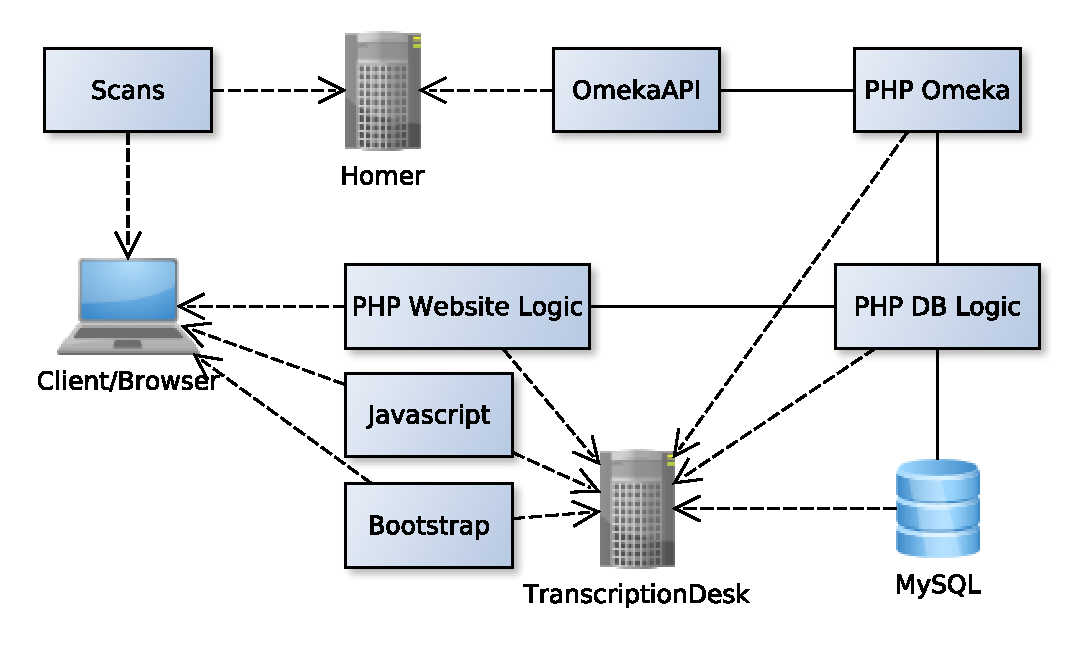
\includegraphics[width=\textwidth]{../notes/components.pdf}
\caption{Diagramm einzelner Komponenten der TranscriptionDesk Website}
\label{fig:components}
\end{figure}

Auf dem Server Homer ist eine Instanz der Omeka\footnote{\url{http://omeka.org/}} software installiert.
Innerhalb dieser Instanz werden die Scans verwaltet, und anderen Teilnehmern im Internet bereit gestellt.
Um Informationen über einzelne Scans,
deren Metadaten, und Sammlungen von Scans verfügbar zu machen,
stellt Omeka eine eigene API bereit,
von der wir mittels der PHP Omeka komponente in regelmäßigen Zeitabständen Daten sammeln.

Die auf der TranscriptionDesk-Installation laufende MySQL Datenbank dient als Speicherplatz für alle anfallenden Informationen,
sie wird gegenüber dem Rest der Website durch die PHP DB Logic Komponente gekapselt,
die aus einer Reihe von Klassen besteht, deren Aufgabe es ist,
Teile der domänenspezifischen Logik und Queries an die Datenbank zusammenzufassen
und für den Rest des PHP codes verwendbar zu machen.

Aufgabe der PHP Website Logic ist es,
aus den vorliegenden Informationen ein Website zusammen zu setzen,
und den zu verwendenden JavaScript code sowie von uns genutzte Teile des Bootstrap frameworks in die Website einzubetten.
Bootstrap und JavaScript sind hier als getrennte Komponenten dargestellt,
da sie sich prinzipiell auch auf andere Server verschieben lassen.

Zum Anzeigen von Scans auf dem Clientgerät baut der Client neben der Verbindung zum TranscriptionDesk Server auch eine Verbindung zu Omeka auf Homer auf,
um die anzuzeigenden Scans zu erhalten.

\subsection{Datenbank}
In diesem Abschnitt widmen wir uns dem Aufbau der Datenbank.
Da wir mit MySQL eine relationale Datenbank einsetzen,
werden anfallende Daten auf einzelne Tabellen verteilt gespeichert,
die zueinander in Relation stehen.

\begin{figure}[H]
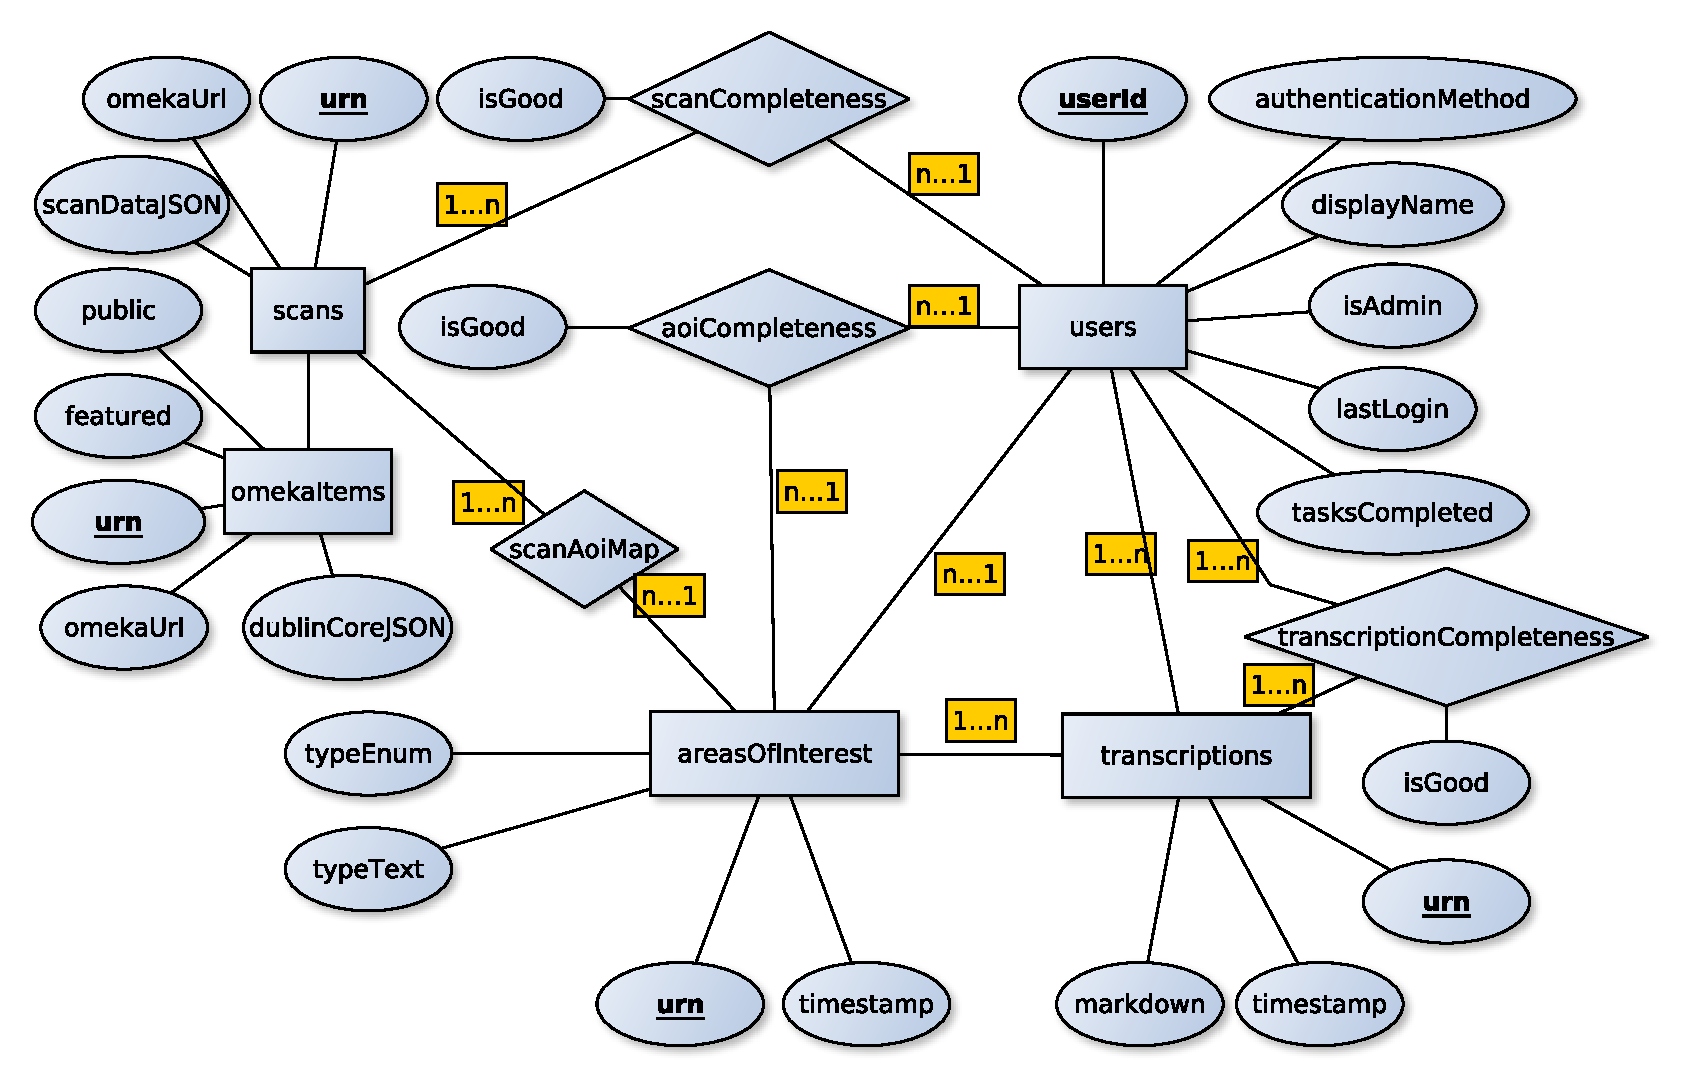
\includegraphics[width=\textwidth]{../notes/ER.pdf}
\caption{Entity-Relationship Diagramm der Datenbank}
\label{fig:er}
\end{figure}

Wie dem Entity-Relationship Diagramm in Abbildung \ref{fig:er} entnommen werden kann,
gibt es in unserer Datenbank 5 Grundlegende Tabellen,
und 4 weitere Tabellen,
die $n:m$ Relationen zwischen diesen realisieren.

\begin{description}
\item[omekaItems:]
    Die Tabelle omekaItems wird von einem systemd timer,
    der die Omekainstanz auf Homer crawled,
    regelmäßig mit Daten befüllt.
    Um eindeutig feststellen zu können,
    welche Datensätze geändert und welche hinzugefügt werden müssen,
    speichern wir dafür sowohl die URL,
    als auch die zugehörige URN jedes Items.
    Um Aufschluss darüber zu haben,
    ob und welchen Besuchern wir bestimmte Datensätze anzeigen dürfen,
    hat jeder Datensatz Booleans in den Feldern public und featured.
    Die von diesen Feldern abgeleitete Zugriffslogik sieht wie folgt aus:

    \begin{tabular}{r|l}
    Nutzer & Bedingung\\\hline
    Unregistrierter Besucher & $\texttt{public}\land\texttt{featured}$\\
    Registrierter Benutzer & $\texttt{featured}$
    \end{tabular}

    Weiterhin gibt es noch das Feld dublinCoreJSON,
    in dem die Dublin Core Daten aus Omeka im JSON Format abgelegt werden.
    Diese Abweichung vom relationalen Paradigma bei Datenbanken wählten wir,
    da die Dublin Core Daten sich teilweise stark unterscheiden,
    und keiner gezielten Selektion durch SQL bedürfen.
\item[scans:]
    In der Tabelle scans sammeln wir die Daten zu allen einzelnen Scans,
    wie wir sie mittels des systemd timers erhalten.
    Genau wie die omekaItems Tabelle hat auch die scans Tabelle Felder für URN und URL.
    Zusätzlich gibt es das Feld scanDataJSON,
    in dem Metadaten zum Scan gesammelt werden.
    Dazu zählen etwa die unterschiedlichen Auflösungen,
    in denen ein Scan verfügbar ist,
    oder das Dateiformat des Scans.
\item[areasOfInterest:]
    Alle von Nutzern der TranscriptionDesk Website markierten Areas of Interest werden in der areasOfInterest Tabelle gespeichert.
    Für jede Area of Interest wird eine eindeutige URN generiert,
    und der Zeitstempel ihrer Erstellung gespeichert.
    Da Areas of Interest einen Typ und in manchen Fällen auch eine Beschreibung haben sollen,
    gibt es in dieser Tabelle die Felder typeEnum und typeText.
\item[transcriptions:]
    Die transcriptions Tabelle ordnet jeder Area of Interest eine Transcription im Markdown format zu,
    sowie den Zeitstempel des speicherns und eine eindeutige URN, die von der der zugehörigen Area of Interest abgeleitet wird.
\item[users:]
    Um Nutzern die Registerierung zu ermöglichen,
    sowie eine einfache Rechteverwaltung zu etablieren,
    gibt es die Tabelle users.
    Jeder Eintrag dieser Tabelle verfügt über eine eindeutige Nummer, die userId.
    Im Feld authenticationMethod speichern wir JSON encodiert Daten,
    die den Authentikationsservice beschreiben,
    und eine eindeutige Zuordnung eines Nutzers zu einem Authentisierungsservice wie z.B. GitHub ermöglichen.
    Um Nutzern einen grundlegenden Grad von Anonymität zu ermöglichen,
    gibt es das Feld displayName,
    in dem der Name des Nutzers eingetragen ist,
    der auf der Seite angezeigt werden soll.
    Wir speichern außerdem im Feld tasksCompleted
    die Anzahl der Aufgaben, die ein Nutzer erledigt hat,
    d.h. die Summe aller erstellten Areas of Interest, Transkriptionen,
    und teilgenommener Abstimmungen.
    Um feststellen zu können, welche Area of Interest oder welche Transkription
    von welchem Nutzer erstellt wurden,
    haben die jeweiligen Tabellen Felder,
    die auf einen Eintrag in der users Tabelle verweisen.
\end{description}

Neben diesen grundlegenden Tabellen sind 3 weitere Tabellen hervorzuheben:
Die Tabellen aoiCompleteness, scanCompleteness und transcriptionCompleteness
realisieren Abstimmungen über die Vollständigkeit der jeweiligen Areas of Interest, Transkriptionen, und scans.
Das bedeutet, dass Nutzer abstimmen können,
für wie gelungen sie eines der jeweiligen Artefakte halten,
und ob sie die Arbeit mit diesem für beendet erklären wollen.
Bei diesen Abstimmungen können Nutzer entweder zustimmen oder ablehnen.
In der Software lässt sich eine Anzahl Stimmen konfigurieren,
die für Zustimmung oder Ablehnung notwendig ist,
und als Entscheidung der Nutzerbasis gewertet wird.
Stimmt ein als Administrator markierter Nutzer ab,
so wird dessen Stimme sofort als Entscheidung gewertet.

\section{Projektverlauf}
In diesem Abschnitt möchten wir den Ablauf unseres Projektes von den ersten Treffen bis hin zum finalen Stand berichten. Dass nicht immer alles planmäßig verläuft liegt in der Natur der Sache. Deswegen möchten wir die unterwegs aufgetretenen Probleme genauer betrachten, und unsere Entscheidungen und Abwägungen nachvollziehbar darlegen. \\
Ausgehend von unseren bereits erwähnten Zielen waren wir zu Beginn in der Lage, notwendige Technologien abzuschätzen. Dabei legten wir viel Wert auf die Auslagerung von Funktionen auf Dienste, welche die benötigte Funktionalität bereits implementiert haben und zur Verfügung stellen und stellten fest, welche Frameworks und Sprachen wir benötigen würden. Danach legten wir die groben Entwicklungsetappen fest, welche bereits in Form unserer drei Meilensteine unter Punkt 3.1. Erwähnung fanden. Die Meilensteine hatten allerdings nicht von Anfang an diese Form. Nur den ersten Meilenstein konnten wir zu diesem Zeitpunkt bereits klar abgrenzen. Uns war klar, dass auch mindestens ein zweiter Meilenstein von Nöten wäre. Dieser hatte zu diesem Zeitpunkt allerdings kaum konkrete Ziele, und die Entstehung eines dritten Meilensteines war zu diesem Zeitpunkt weder angedacht noch ausgeschlossen worden. Zwischenzeitlich wurde sogar ein vierter Meilenstein geplant, doch unser erster Meilenstein erfüllte letzten Endes mehr Anforderungen als geplant, so dass sich die Planung nach hinten wieder anders gestaltete.
Wir wussten zu Beginn, dass die Scans auf einem Fileserver liegen, was aus rechtlichen Gründen aber nicht so bleiben sollte. An diesem Punkt gab es noch keine konkrete Antwort auf die Frage, von wo wir die Bilder beziehen, und wie wir entsprechend darauf zugreifen könnten. Außerdem waren wir uns schon einig, dass wir, in Anlehnung an das Homer-Multitext-Projekt, ebenfalls Areas of Interest verwenden möchten, welche im dortigen Projekt als ,,Regions of Interest'' bezeichnet werden. Wir waren uns auch einig, dass Rechtecke die optimale Form wären, um diese Regionen zu markieren, wussten nur noch nicht mit Sicherheit, inwelcher Form wir diese Umsetzen und abspeichern sollten. Unser Favorit war die Variante, dass Rechtecke nur parallel zu den Seiten verlaufen könnten und man lediglich zwei Punkte, oder einen Punkt sowie Höhe und Breite abspeichern müsste. Nach kurzer Bedenkzeit entschieden wir uns für die zuletzt genannte Variante. Außerdem waren wir schon zu Beginn darüber im Bilde, dass Nutzer sich in irgendeiner Form Registrieren können sollten, und dass dies eine Voraussetzung wäre, um auf die Daten zugreifen zu können. Deswegen war die Login-Routine eine der ersten beschlossenen Funktionen. Außerdem war ebenfalls klar, dass Arbeit nur im eingeloggten Zustand verrichtet werden darf. \\
Eine Woche später kam Omeka als Server für unsere Bilddateien ins Gespräch. Dort sollten wir einen Contributor-Nutzerzugang bekommen um über diesen Zugang zu den Scans zu erhalten. Schnell stellte sich auch die Frage, ob wir ein Omeka-Plugin bauen müssten, oder ob es hierfür bereits implementierte Instrumente gäbe, deren Verwendung für uns in Frage kommt. Noch am selben Tag entschlossen wir uns dazu, für die Anmeldung einen Authentification Provider zu verwenden.

%Virtual Machine/Containerlösung: Zuerst Docker, dann Vagrant, weil schwierig unter Windows einzurichten. BootToDocker sollte auf Windows laufen, war allerdings kaputt und lief unter Windows nicht. Weitere Probleme wurden erwartet. Deswegen Wechsel zu Vagrant.
%MUFI-Keyboard: Franz hat zuerst eine Eingabemaske dafür entwickelt. Allerdings ist es schwierig zu organisieren, da MUFI unglaublich viele Symbole hat. Eine günstigere Organisierung war notwendig. Wechsel der Technik war schwierig zu planen. MUFI-Symbole waren vorher in MUFI-vorgegebenen Kategorien organisiert, diese machten keinen Sinn für die Eingabemaske. Eigene Kategorisierung der Symbole wurde notwendig. Die substrings der Description eines Zeichens wurden als Tags verwendet. Diese wurden mittels Bucket-Sort organisiert und bessere Kategorien entstanden.

\subsection{Aktueller Stand des Projektes}

\section{Zusammenfassung und Ausblick}

\section*{Quellen}
  \printbibliography[%
    heading=bibintoc, % (bibintoc, bibnumbered)
  ]
\end{document}
